
\documentclass[compress,red]{beamer}
\mode<presentation>

\usetheme{Warsaw}

% define your own colours:
\definecolor{Red}{rgb}{1,0,0}
\definecolor{Blue}{rgb}{0,0,1}
\definecolor{Green}{rgb}{0,1,0}
\definecolor{magenta}{rgb}{1,0,.6}
\definecolor{lightblue}{rgb}{0,.5,1}
\definecolor{lightpurple}{rgb}{.6,.4,1}
\definecolor{gold}{rgb}{.6,.5,0}
\definecolor{orange}{rgb}{1,0.4,0}
\definecolor{hotpink}{rgb}{1,0,0.5}
\definecolor{newcolor2}{rgb}{.5,.3,.5}
\definecolor{newcolor}{rgb}{0,.3,1}
\definecolor{newcolor3}{rgb}{1,0,.35}
\definecolor{darkgreen1}{rgb}{0, .35, 0}
\definecolor{darkgreen}{rgb}{0, .6, 0}
\definecolor{darkred}{rgb}{.75,0,0}

\xdefinecolor{olive}{cmyk}{0.64,0,0.95,0.4}
\xdefinecolor{purpleish}{cmyk}{0.75,0.75,0,0}

% \usepackage{beamerinnertheme_______}
% inner themes include circles, default, inmargin, rectangles, rounded

%\usepackage{beamerouterthemesmoothbars}
% outer themes include default, infolines, miniframes, shadow, sidebar, smoothbars, smoothtree, split, tree

\useoutertheme[subsection=false]{smoothbars}

% to have the same footer on all slides
%\setbeamertemplate{footline}[text line]{xxx xxx xxx}
%\setbeamertemplate{footline}[text line]{} % or empty footer

% include packages
\usepackage{subfigure}
\usepackage{multicol}
\usepackage{amsmath}
\usepackage{epsfig}
\usepackage{graphicx}
\usepackage[all,knot]{xy}
\xyoption{arc}
\usepackage{url}
\usepackage{multimedia}
\usepackage{hyperref}
\usepackage{setspace}

\title{A bottom up sensor testbed}
\subtitle{Hands on WSN}
\author{Sergio Almendros Diaz}
\institute[institute]{Universitat Pompeu Fabra}
\date[date]{February, 2014, Barcelona}

\begin{document}

\frame{
	\titlepage
}

%\section[Outline]{}
%\frame{\tableofcontents}

\section{General overview of the project}
   
  \subsection{Goals}
  \frame{\frametitle{Goals}
  The \textbf{general goals} of my project can be summarised in the following points:
  \vspace{0.25cm}
  \begin{enumerate}
  \item Gather \textbf{data} about temperature, humidity, light, noise, and air quality.
  \vspace{0.25cm}
  \item \textbf{Share} the data as open data.
  \vspace{0.25cm}
  \item \textbf{Visualize} the data in a Android application.
  \end{enumerate}
  }
  
  \subsection{Introduction}
  \frame{\frametitle{Introduction}
  This project has two main parts:
  \vspace{0.25cm}
  \begin{enumerate}
  \item \textbf{Arduino YUN}. \\
  \begin{center} 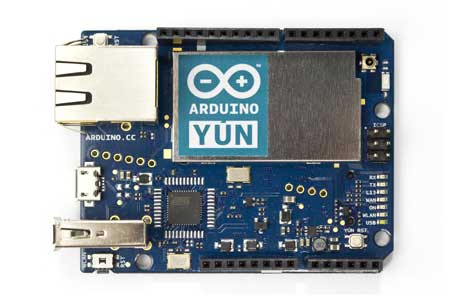
\includegraphics[scale=.2]{figures/ArduinoYunFront_2_450px.jpg} \end{center}
  \item \textbf{Android app}. \\
  \begin{center} 
\includegraphics[scale=0.05]{figures/Android-logo.png} \end{center}
  \end{enumerate}
  }

\section{Arduino Code}
\frame{\frametitle{Arduino Code}
The arduino code has three functionalities:
  \vspace{0.25cm}
\begin{enumerate}
\item \textbf{Collect} the analog \& digital data. \\
  \begin{center} 
    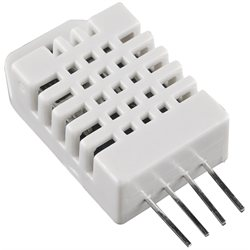
\includegraphics[scale=.2]{figures/dht22.jpg} 
    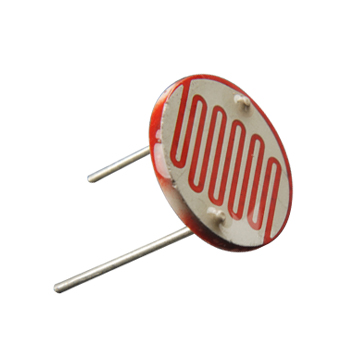
\includegraphics[scale=.2]{figures/LDR.jpg} 
    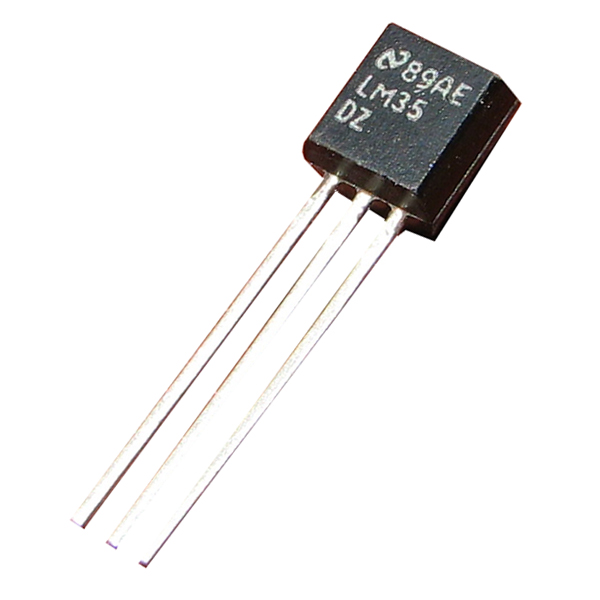
\includegraphics[scale=.2]{figures/LM35.jpg} 
    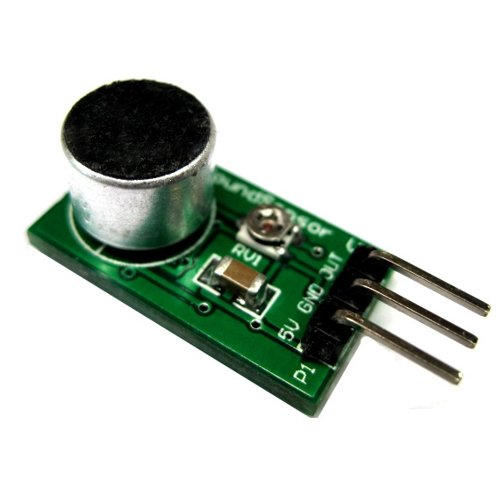
\includegraphics[scale=.2]{figures/MiniSoundSensor.jpg} 
    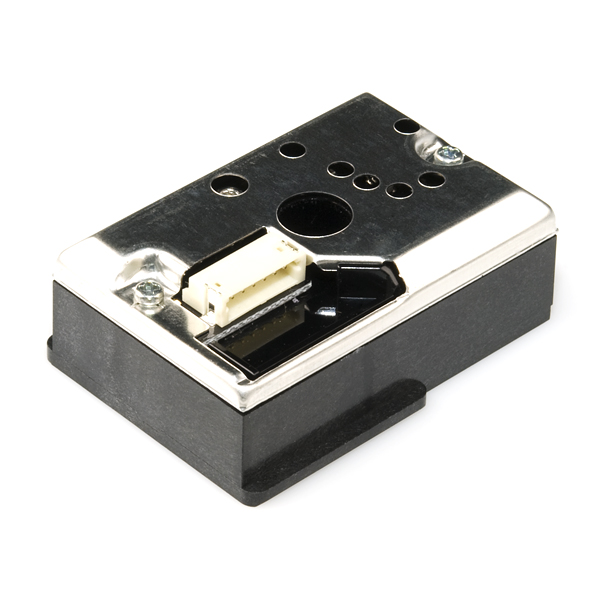
\includegraphics[scale=.2]{figures/sharp.jpg} 
  \end{center}
\vspace{0.25cm}
\item Write it in the \textbf{logData} file.
\vspace{0.25cm}
\item Call the \textbf{python script} with the sensory data as arguments, and then the script will send it to opencities. \\
\begin{center} 
    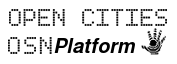
\includegraphics[scale=.6]{figures/logo.png} 
  \end{center}
\end{enumerate}
}

\section{Android App}
\frame{\frametitle{Android App}
The app should do:
  \vspace{0.25cm}
\begin{enumerate}
\item Get the \textbf{real-time} data from opencities. \\
\vspace{0.25cm}
\item Show it in a way that anybody can \textbf{understand} it.
\end{enumerate}
}


\section*{}
\frame{
    \begin{center}
        \begin{huge}
        Thank you for your attention.
        \end{huge}
        \\
        \vspace{1cm}
        Reporsitory at github.com/SergioAlmendros/A-bottom-up-sensor-testbed \\ 
        \pause
        \vspace{1cm}
        \begin{huge}
        Any questions?
        \end{huge}
    \end{center}
}

\end{document} 
